%-%-%-%-%-%-%-%-%-%-%-%-%-%-%-%-%-%-%-%-%-%-%-%-%-%-%-%-%-%-%-%-%-%-%-%-%-%-%
%This is a blank document for homework assignments.

%Some preliminaries:  Anything after a '%' is a comment - it isn't read by 
%the compiler.  

%You are welcome to skip down to lines 38-44 to put in some information, and 
%then to line 57 to start writing, but the preamble contains all the 
%formatting that makes it look nice, if you're interested in how that works.

%Packages are just collections of commands to do different things.  For
%almost anything you might want to do, there's a package that will do it.
%-%-%-%-%-%-%-%-%-%-%-%-%-%-%-%-%-%-%-%-%-%-%-%-%-%-%-%-%-%-%-%-%-%-%-%-%-%-%


\documentclass[12pt]{article}  
%The article class is a very basic type of document for writing
%We will customize it to do what we want.

\usepackage[margin=1in]{geometry}  %Adjust margins, formatting

\usepackage{amsmath}  
\usepackage{amssymb}  
\usepackage{amsfonts}  
%These packages add commands for useful symbols and fonts and things like that.
%Most of the time, these are all you need.

\usepackage{textcomp, gensymb}  %Gives more symbols, like /degree

\usepackage{amsthm}

\usepackage{fancyhdr}  %Header and Footer formatting
\pagestyle{fancy}  
\renewcommand{\headrulewidth}{0.4pt}
\renewcommand{\footrulewidth}{0.4pt}
\setlength{\headheight}{18pt}

%Header and Footer Information
\lhead{\large{\bf Murphy}}  %Replace with your name
\chead{}
\rhead{\textsc{Unprepared class day}}  %Replace "Title" with the name of the assignment
\lfoot{\today}  %You can let it put in today's date or put one in yourself
\cfoot{}
\rfoot{\thepage\ of \ref{NumPages}}  %Counts the pages.

\makeatletter        %This provides a total page count as \ref{NumPages}                 
\AtEndDocument{\immediate\write\@auxout{\string\newlabel{NumPages}{{\thepage}}}}
\makeatother

\usepackage{amsthm}  %This will create the Problem environment
\theoremstyle{definition}
\newtheorem{problem}{Problem}
\renewcommand*{\proofname}{Solution}

\usepackage{graphicx}

\begin{document}



\begin{problem}
Murphy wants me to type up some stuff from page 599. And so I'm going to include Figure \ref{fig:Jam1}.

\begin{proof}
Let's include an image first, just for fun.

\begin{figure}[h]
    \centering
    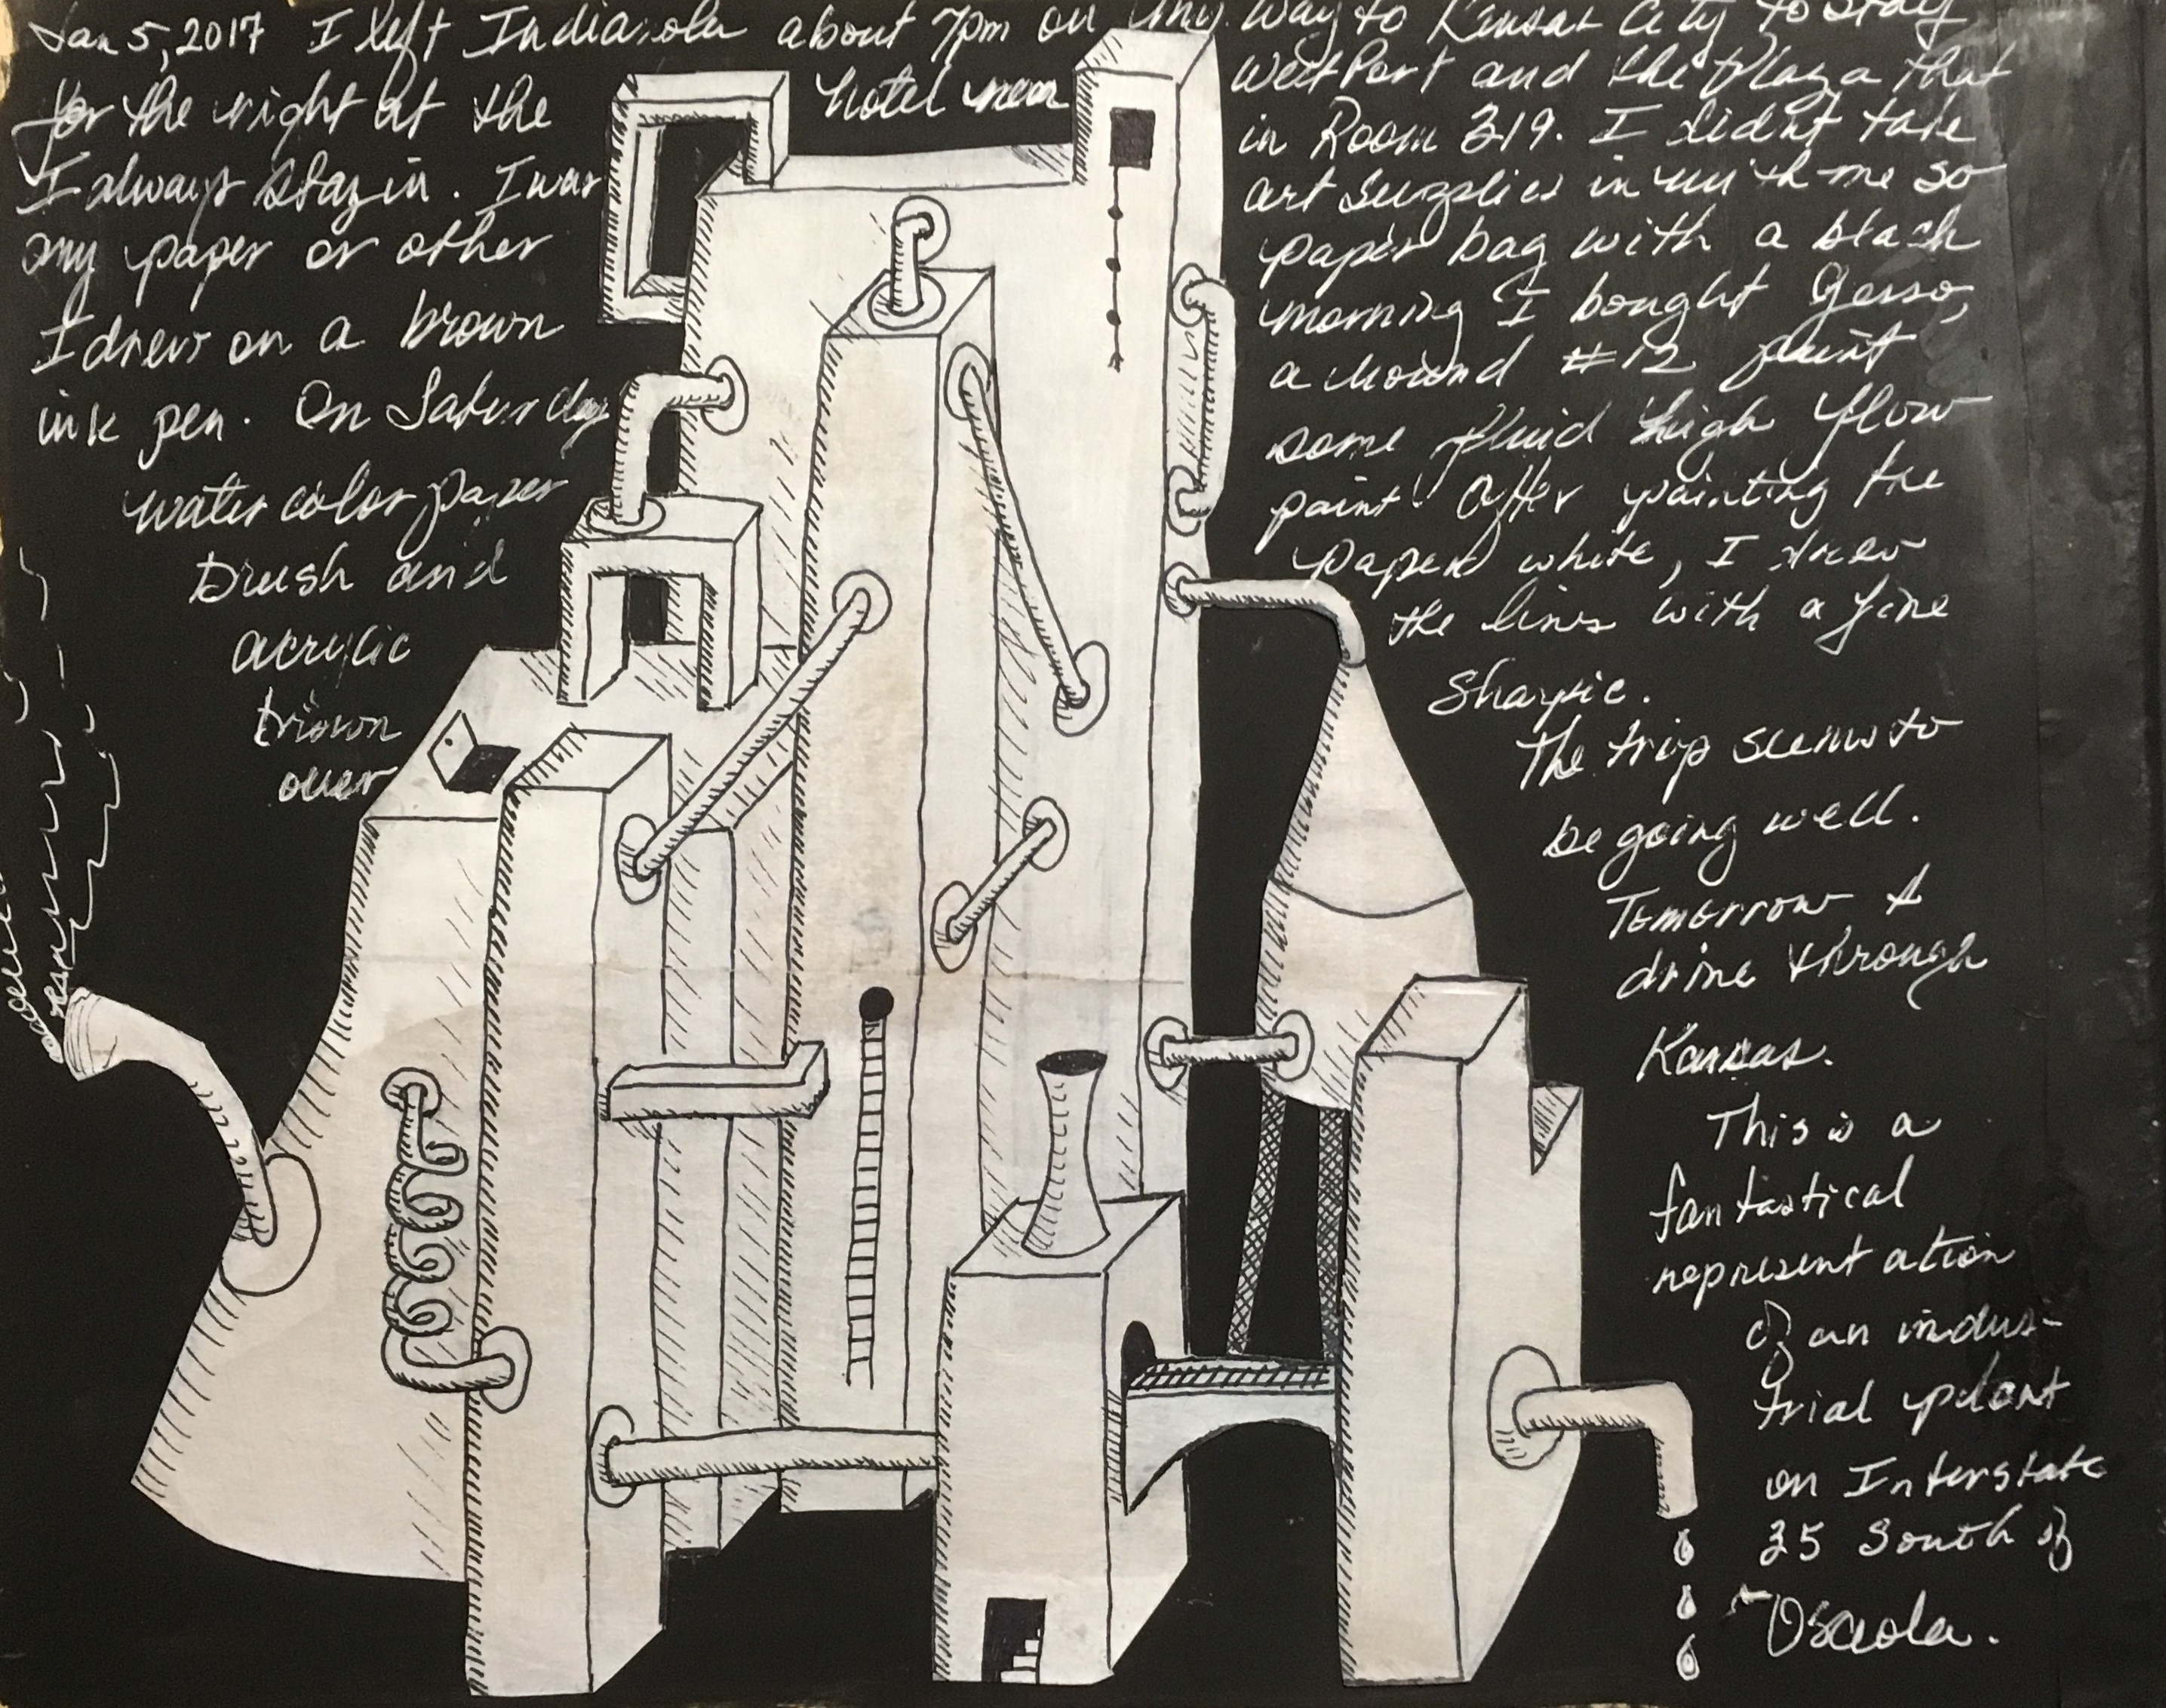
\includegraphics[width=0.5\textwidth]{Week1Jamie1.jpg}
    \caption{8" x 11" mixed media collage}
    \label{fig:Jam1}
\end{figure}

What 
if I 
type
something                            like this.

If I want an inline equation I use $y = x + 1$.  But if I want a centered equation I use $$y = x + 1$$ and it puts it on its own line. Maybe I want to refer to Equation \ref{eqn:simple}.

This is another equation
\begin{equation}
    \label{eqn:simple}
    y = \frac{x^{5e} + 1}{\partial x}
\end{equation}
embedded in a sentence.

This is another equation
\begin{align} 
2x - 5y &=  8 ,&x > 2\\    3x + 9y &=  -12 ,& y <1
\end{align}

embedded in a sentence.

And then we'll do some other stuff.
\end{proof}
\end{problem}

\end{document}